% [fig-q18-rhombus], fixed PDF p.1 / printed 963.
% These are page-layout projections, not spatial coordinates or derived edges.
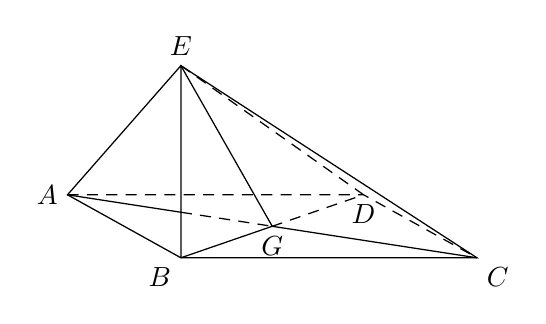
\begin{tikzpicture}[line width=.45pt,scale=.8]
  \coordinate (A) at (0,1);
  \coordinate (B) at (1.8,0);
  \coordinate (C) at (6.5,0);
  \coordinate (D) at (4.7,1);
  \coordinate (G) at (3.25,.5);
  \coordinate (E) at (1.8,3.05);
  \draw (E) -- (A) -- (B) -- (C) -- (E) -- (B);
  \draw (E) -- (G) -- (C) (B) -- (G);
  % Source AC is solid from A to EB, hidden from EB to G, solid G to C.
  \draw (A) -- (1.8,.72308);
  \draw[dash pattern=on 4pt off 3pt] (1.8,.72308) -- (G);
  \draw[dash pattern=on 4pt off 3pt] (A) -- (D) -- (C) (E) -- (D) -- (G);
  \node[left] at (A) {$A$};
  \node[below left] at (B) {$B$};
  \node[below right] at (C) {$C$};
  \node[below] at (D) {$D$};
  \node[above] at (E) {$E$};
  \node[below] at (G) {$G$};
\end{tikzpicture}
